\documentclass{article}
\usepackage{tikz}

\begin{document}

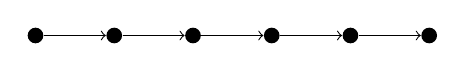
\begin{tikzpicture}[node distance=1cm]
    \foreach \x in {1,...,6} {
        \node[circle,fill,inner sep=2pt] (p\x) at (\x,0) {};
    }
    \draw[->] (p1) -- (p2);
    \draw[->] (p2) -- (p3);
    \draw[->] (p3) -- (p4);
    \draw[->] (p4) -- (p5);
    \draw[->] (p5) -- (p6);
\end{tikzpicture}

\end{document}